% Options for packages loaded elsewhere
\PassOptionsToPackage{unicode}{hyperref}
\PassOptionsToPackage{hyphens}{url}
\PassOptionsToPackage{dvipsnames,svgnames,x11names}{xcolor}
%
\documentclass[
]{jds}

\usepackage{amsmath,amssymb}
\usepackage{iftex}
\ifPDFTeX
  \usepackage[T1]{fontenc}
  \usepackage[utf8]{inputenc}
  \usepackage{textcomp} % provide euro and other symbols
\else % if luatex or xetex
  \usepackage{unicode-math}
  \defaultfontfeatures{Scale=MatchLowercase}
  \defaultfontfeatures[\rmfamily]{Ligatures=TeX,Scale=1}
\fi
\usepackage{lmodern}
\ifPDFTeX\else  
    % xetex/luatex font selection
\fi
% Use upquote if available, for straight quotes in verbatim environments
\IfFileExists{upquote.sty}{\usepackage{upquote}}{}
\IfFileExists{microtype.sty}{% use microtype if available
  \usepackage[]{microtype}
  \UseMicrotypeSet[protrusion]{basicmath} % disable protrusion for tt fonts
}{}
\makeatletter
\@ifundefined{KOMAClassName}{% if non-KOMA class
  \IfFileExists{parskip.sty}{%
    \usepackage{parskip}
  }{% else
    \setlength{\parindent}{0pt}
    \setlength{\parskip}{6pt plus 2pt minus 1pt}}
}{% if KOMA class
  \KOMAoptions{parskip=half}}
\makeatother
\usepackage{xcolor}
\setlength{\emergencystretch}{3em} % prevent overfull lines
\setcounter{secnumdepth}{-\maxdimen} % remove section numbering
% Make \paragraph and \subparagraph free-standing
\ifx\paragraph\undefined\else
  \let\oldparagraph\paragraph
  \renewcommand{\paragraph}[1]{\oldparagraph{#1}\mbox{}}
\fi
\ifx\subparagraph\undefined\else
  \let\oldsubparagraph\subparagraph
  \renewcommand{\subparagraph}[1]{\oldsubparagraph{#1}\mbox{}}
\fi


\providecommand{\tightlist}{%
  \setlength{\itemsep}{0pt}\setlength{\parskip}{0pt}}\usepackage{longtable,booktabs,array}
\usepackage{calc} % for calculating minipage widths
% Correct order of tables after \paragraph or \subparagraph
\usepackage{etoolbox}
\makeatletter
\patchcmd\longtable{\par}{\if@noskipsec\mbox{}\fi\par}{}{}
\makeatother
% Allow footnotes in longtable head/foot
\IfFileExists{footnotehyper.sty}{\usepackage{footnotehyper}}{\usepackage{footnote}}
\makesavenoteenv{longtable}
\usepackage{graphicx}
\makeatletter
\def\maxwidth{\ifdim\Gin@nat@width>\linewidth\linewidth\else\Gin@nat@width\fi}
\def\maxheight{\ifdim\Gin@nat@height>\textheight\textheight\else\Gin@nat@height\fi}
\makeatother
% Scale images if necessary, so that they will not overflow the page
% margins by default, and it is still possible to overwrite the defaults
% using explicit options in \includegraphics[width, height, ...]{}
\setkeys{Gin}{width=\maxwidth,height=\maxheight,keepaspectratio}
% Set default figure placement to htbp
\makeatletter
\def\fps@figure{htbp}
\makeatother

\makeatletter
\@ifpackageloaded{caption}{}{\usepackage{caption}}
\AtBeginDocument{%
\ifdefined\contentsname
  \renewcommand*\contentsname{Table of contents}
\else
  \newcommand\contentsname{Table of contents}
\fi
\ifdefined\listfigurename
  \renewcommand*\listfigurename{List of Figures}
\else
  \newcommand\listfigurename{List of Figures}
\fi
\ifdefined\listtablename
  \renewcommand*\listtablename{List of Tables}
\else
  \newcommand\listtablename{List of Tables}
\fi
\ifdefined\figurename
  \renewcommand*\figurename{Figure}
\else
  \newcommand\figurename{Figure}
\fi
\ifdefined\tablename
  \renewcommand*\tablename{Table}
\else
  \newcommand\tablename{Table}
\fi
}
\@ifpackageloaded{float}{}{\usepackage{float}}
\floatstyle{ruled}
\@ifundefined{c@chapter}{\newfloat{codelisting}{h}{lop}}{\newfloat{codelisting}{h}{lop}[chapter]}
\floatname{codelisting}{Listing}
\newcommand*\listoflistings{\listof{codelisting}{List of Listings}}
\makeatother
\makeatletter
\makeatother
\makeatletter
\@ifpackageloaded{caption}{}{\usepackage{caption}}
\@ifpackageloaded{subcaption}{}{\usepackage{subcaption}}
\makeatother
\ifLuaTeX
  \usepackage{selnolig}  % disable illegal ligatures
\fi
\usepackage[]{natbib}
\bibliographystyle{plainnat}
\usepackage{bookmark}

\IfFileExists{xurl.sty}{\usepackage{xurl}}{} % add URL line breaks if available
\urlstyle{same} % disable monospaced font for URLs
\hypersetup{
  pdftitle={My wonderful paper},
  colorlinks=true,
  linkcolor={blue},
  filecolor={Maroon},
  citecolor={Blue},
  urlcolor={Blue},
  pdfcreator={LaTeX via pandoc}}

\title{My wonderful paper}
\author{}
\date{}

\begin{document}
\maketitle
\begin{abstract}
This is the abstract
\end{abstract}

\section{Introduction}\label{introduction}

{[}background{]}

In this paper, a concept called analysis plan is proposed to describe
the logical structure of a data analysis. An analysis plan is a set of
analysis steps plus their expected outcomes. It is a formal
representation of the analysis process and can be used to guide the
analysis process, to communicate and compare the analysis process to
others, and to evaluate the analysis process. The concept of analysis
plan is illustrated with examples. The implications of the concept for
data analysis practice is discussed.

The analysis plan described in this paper should be differentiated from
the pre-specifies analysis plan document often used in biostatistics to
specifies the hypothesis, data collection mechanism, statistical
procedures etc of randomized experiments.

The rest of the paper is organized as follows: Section~\ref{sec-plan}
describes the concept of analysis plan in detail.
Section~\ref{sec-examples} provides examples of analysis plan {[}more
details{]}. (need another section here or before examples?)
Section~\ref{sec-conclusion} concludes the paper.

\section{Analysis plan}\label{sec-plan}

\begin{itemize}
\item
  describe/ define what analysis plan is, expectation (outcome and plan)
\item
  why it is useful to be explicit about expectation?

  \begin{itemize}
  \tightlist
  \item
    expectations can be used to formulate unit tests, which helps to
    divide the ``result universe''
  \end{itemize}
\end{itemize}

\section{Examples}\label{sec-examples}

Three examples are presented to illustrate how the concept of analysis
plan can be applied to data analysis. {[}toy example{]}.
Section~\ref{sec-linear-reg} illustrates how constructing the result
universe in a linear regression model of PM10 on mortality can help
understand the impact of sample size, model specification, and variable
correlation structure on data analysis. {[}example three{]}

\subsection{A toy example}\label{a-toy-example}

\subsection{Linear regression}\label{sec-linear-reg}

Consider a linear regression model to study the effect of PM10 on
mortality (provide context of using PM10 to study mortality). Analysts
may expect a significant (p-value \(\le\) 0.05) PM10 coefficient in the
linear model from the literature. This is the \emph{outcome
expectation}. There are multiple factors that can affect the outcome
expectation of linear regression, which here is called \emph{plan
expectation}, for example, 1) sample size, 2) model specification, and
3) correlation structure between variables. Adequate sample size is
required to achieve the desired power to detect the significance of PM10
on mortality. Temperature is often an important confounder to consider
in such study (add reference). From some domain knowledge, an analyst
may expect that the significance of PM10 coefficient can be attained by
adding temperature to the model. Analysts may also expect certain
correlation structure between PM10, temperature, and mortality, and the
distribution of each variable.

To build the result universe, datasets can be simulated to either meet
and fail these plan expectations, allowing the analysts to observe the
significance of PM10 coefficient. Here, sample sizes of 50, 100, 500,
and 1000 are considered. Two model specifications are included: 1)
linear model with PM10 as the only covariate
(\(\text{mortality} \sim \text{PM10}\)), 2) linear model with PM10 and
temperature as covariates
(\(\text{mortality} \sim \text{PM10} + \text{temp}\)). A grid-based
approach is used to simulate correlation structure. Reasonable ranges of
correlation between the three variables are
\(\text{cor}(\text{mortality}, \text{PM10}) \in [-0.01, 0]\),
\(\text{cor}(\text{mortality}, \text{temperature}) \in [-0.6, -0.2]\),
and \(\text{cor}(\text{PM10}, \text{temperature}) \in [0.2, 0.6]\).

\begin{itemize}
\item
  add a paragraph to describe the simulation process
\item
  add a fourth panel to describe the comparison of a right/ wrong
  expectation, i.e.~correlation on PM10 and mortality
\end{itemize}

Figure~\ref{fig-result-universe} shows that result universe of the
linear regression model and how a change of decision in one of the plan
expectations above affect the outcome expectation. Panel a) is colored
by the outcome expectation -- whether a significant p-value is found in
the PM10 coefficient. Panel b) shows the effect of adding temperature to
the model and the results show that the significance of PM10 coefficient
can be achieved by adding temperature to the model for a sample size of
500. Panel c) shows that increasing sample size from 50 to 100 enhances
the significance of p-value for PM10 and the significance remains with
further increases in sample size. {[}note: weave the ``actual data''
into the example linear regression model{]}

(these two paragraphs may go to a new section \emph{discussion}) A
result universe constructed in this example can be presented to analysts
to answer the what-if questions raised in the data analysis. What if the
sample size is increased? What if temperature is added to the model?
What would the results expect to be changed when the correlation
structure is different? For analysts, expectations can be used as unit
tests to divide the result universe, which allows them to understand the
impact of each factor on the outcome expectation.

The result universe also provides a holistic view of how the results
obtained by the analysts are situated in all possible results. This can
be seen as a direct towards trustworthy data analysis, where the
audience of the analysis to exercise their own cognitive model
\citep{grolemund_cognitive_2014} to evaluate the results reported.

\textsubscript{Source:
\href{https://huizezhang-sherry.github.io/paper-analysis-plan/index.qmd.html}{Article
Notebook}}

\phantomsection\label{cell-fig-result-universe}
\begin{figure}[H]

\centering{

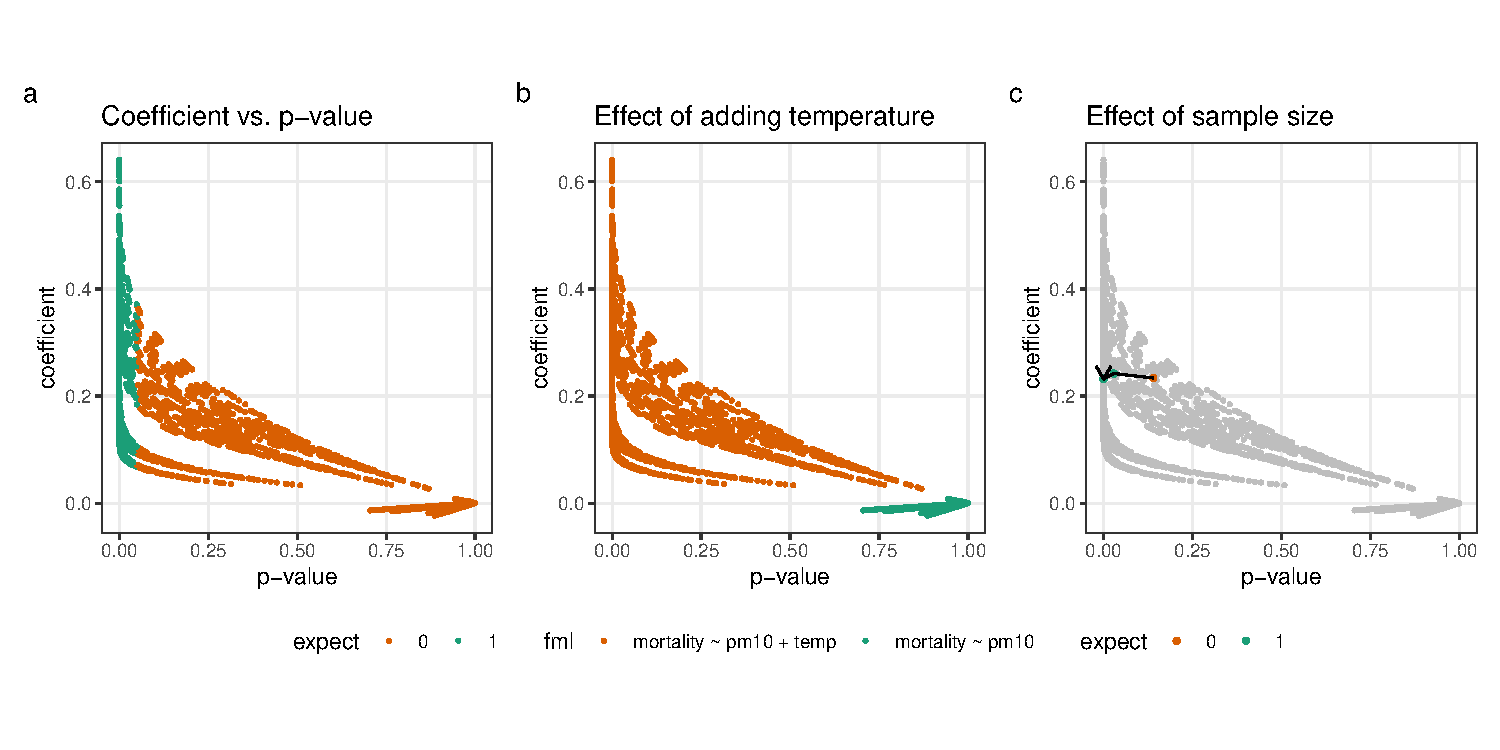
\includegraphics{index_files/figure-pdf/fig-result-universe-1.pdf}

}

\caption{\label{fig-result-universe}The result universe of linear
regression model to study the effect of PM10 on mortality: a) colored by
whether the p-value of PM10is significant (less than 0.05), b) the
effect of adding temperature to the model for a sample size of 500, c)
the effect of increasing sample size for a fixed correlation structure.}

\end{figure}%

\textsubscript{Source:
\href{https://huizezhang-sherry.github.io/paper-analysis-plan/index.qmd.html}{Article
Notebook}}

\section{Conclusion}\label{sec-conclusion}


\renewcommand\refname{References}
  \bibliography{references.bib}


\end{document}
